\documentclass[a4paper, 10pt]{article}
\usepackage[english,brazil]{babel}
\usepackage[utf8]{inputenc}
\usepackage{fullpage}
\usepackage{float}

% \usepackage{multicol}
\usepackage{graphicx}
\usepackage{listings}
% \setlength{\columnsep}{30pt}
% I want the columnsep to be wider only on this page. Right now, nothing happens. The default 10pt is still being used.

\lstdefinestyle{cppStyle}{
  basicstyle=\footnotesize,
  breakatwhitespace=false,
  breaklines=true,
  captionpos=b,
  keepspaces=true,
  numbers=left,
  numbersep=5pt,
  showspaces=false,
  showstringspaces=false,
  showtabs=false,
  tabsize=2
}

% \lstdefinestyle{es}{
%   basicstyle=\footnotesize,
%   breakatwhitespace=false,
%   breaklines=true,
%   captionpos=b,
%   keepspaces=true,
%   numbers=left,
%   numbersep=5pt,
%   showspaces=false,
%   showstringspaces=false,
%   showtabs=false,
%   tabsize=2
% }

\renewcommand*{\lstlistingname}{Código}

\newcounter{codeNum}
\setcounter{codeNum}{0}

\begin{document}

\noindent
\large
\textbf{Compiladores} \\
\textbf{2ª Série de Exercícios} \\
\normalsize CES-41  \\
Professor: Fábio Carneiro Mokarzel \\
Aluno: Carlos Matheus Barros da Silva \hfill Julho de 2019 \\ \\


%-------------------------------------------------------------------------------

\section*{Exercício 1}

O Exercicio foi resolvido com sucesso. De acordo com a gramática Seção 5.5.3 do Capítulo V dos Slides Teóricos de CES-41 e as tabelas de ações e de transições do analisador LR, no mesmo exemplo foi desenvolvido um código em Python que constroi a tabela de execução para uma data sentença.

Portando, dado a sentença $id * ((id + id) * ((id + id) * id)) \$$, a sua tabela de execução pode ser vista na tabela representada pela Figura \ref{fig:tabela}.

\begin{figure}[H]
  \begin{center}
  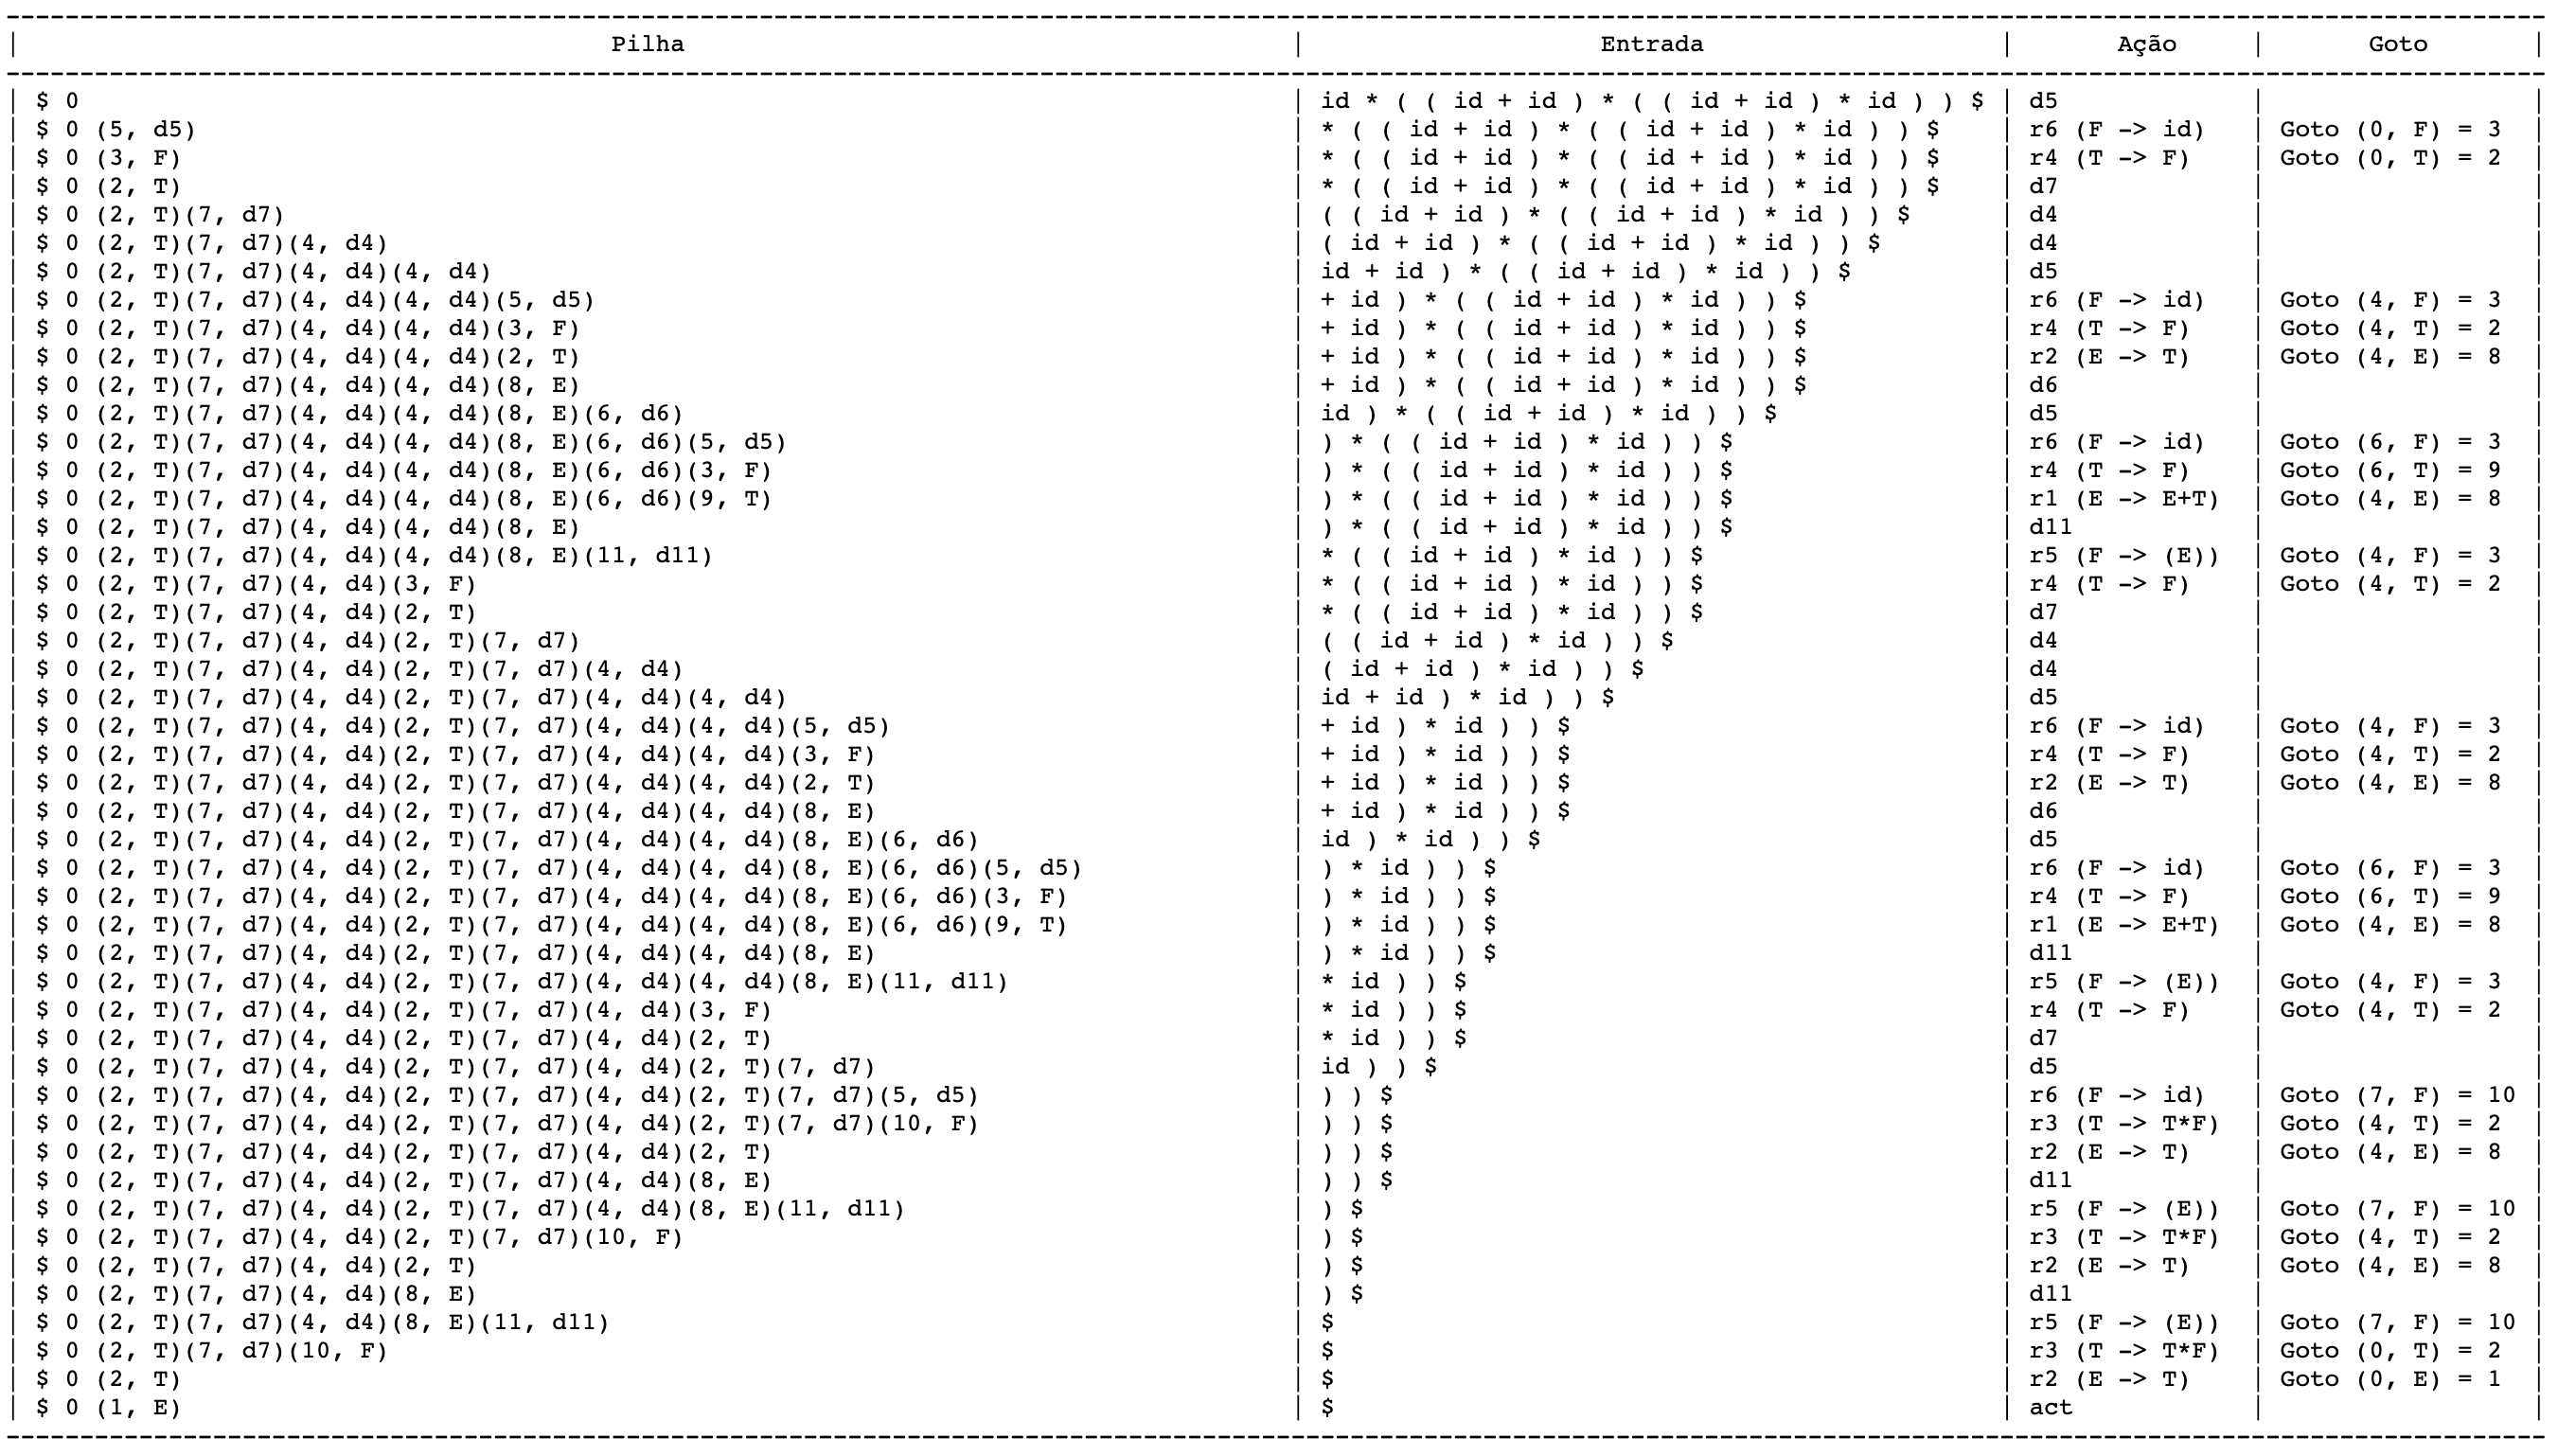
\includegraphics[width=\linewidth]{./../tabela.png}
  \caption{Tabela de execução para entrada $id * ((id + id) * ((id + id) * id)) \$$}
  \label{fig:tabela}
  \end{center}
\end{figure}

\section*{Exercício 2}

O Exercicio foi resolvido com sucesso. Para as produções da gramática:
\begin{center}
    $E  \to  E + T | T$ \\
    $T  \to  T * F | F$ \\
    $F  \to  P @ F | P$ \\
    $P  \to  ( E ) | a | a ( L )$ \\
    $L  \to  L , E | E$ \\
\end{center}
Seus automatos podem ser verificados nas imagens representadas pela Figura \ref{fig:naodeterministico} e pela Figura \ref{fig:deterministico}.

\section*{Exercício 3}

O Exercicio foi resolvido com sucesso. O código intermediário pode ser visto no Código \ref{code:intermediario}

\lstinputlisting[
    language=c,
    caption={Código intermediário livre de quádruplas de operadores NOP e de operadores de atribuição desnecessários},
    label={code:intermediario},
    style=cppStyle,
    numbers=none,
]{./../list2_question3_answer.txt}

\begin{figure}[H]
  \begin{center}
  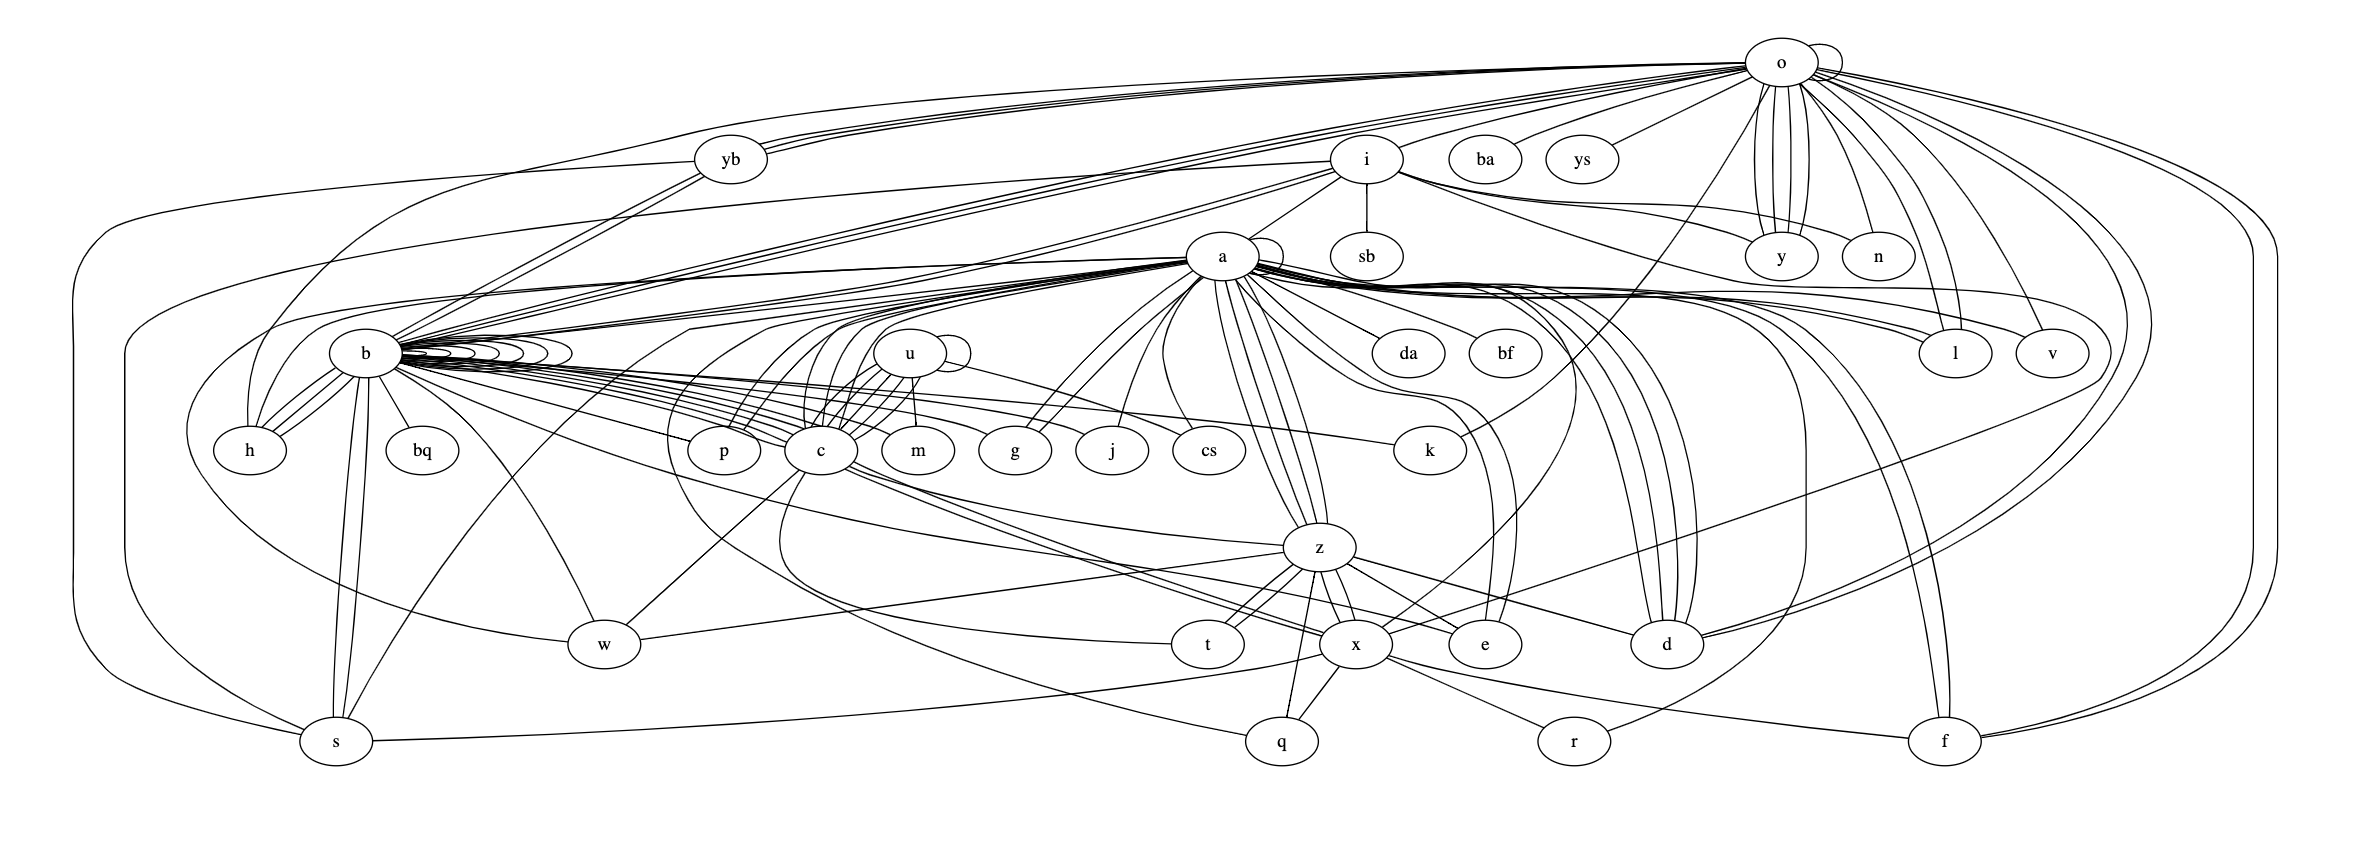
\includegraphics[width=\linewidth]{./../nao_deterministico.png}
  \caption{Automato Finito Não Determinístico}
  \label{fig:naodeterministico}
  \end{center}
\end{figure}

\begin{figure}[H]
  \begin{center}
  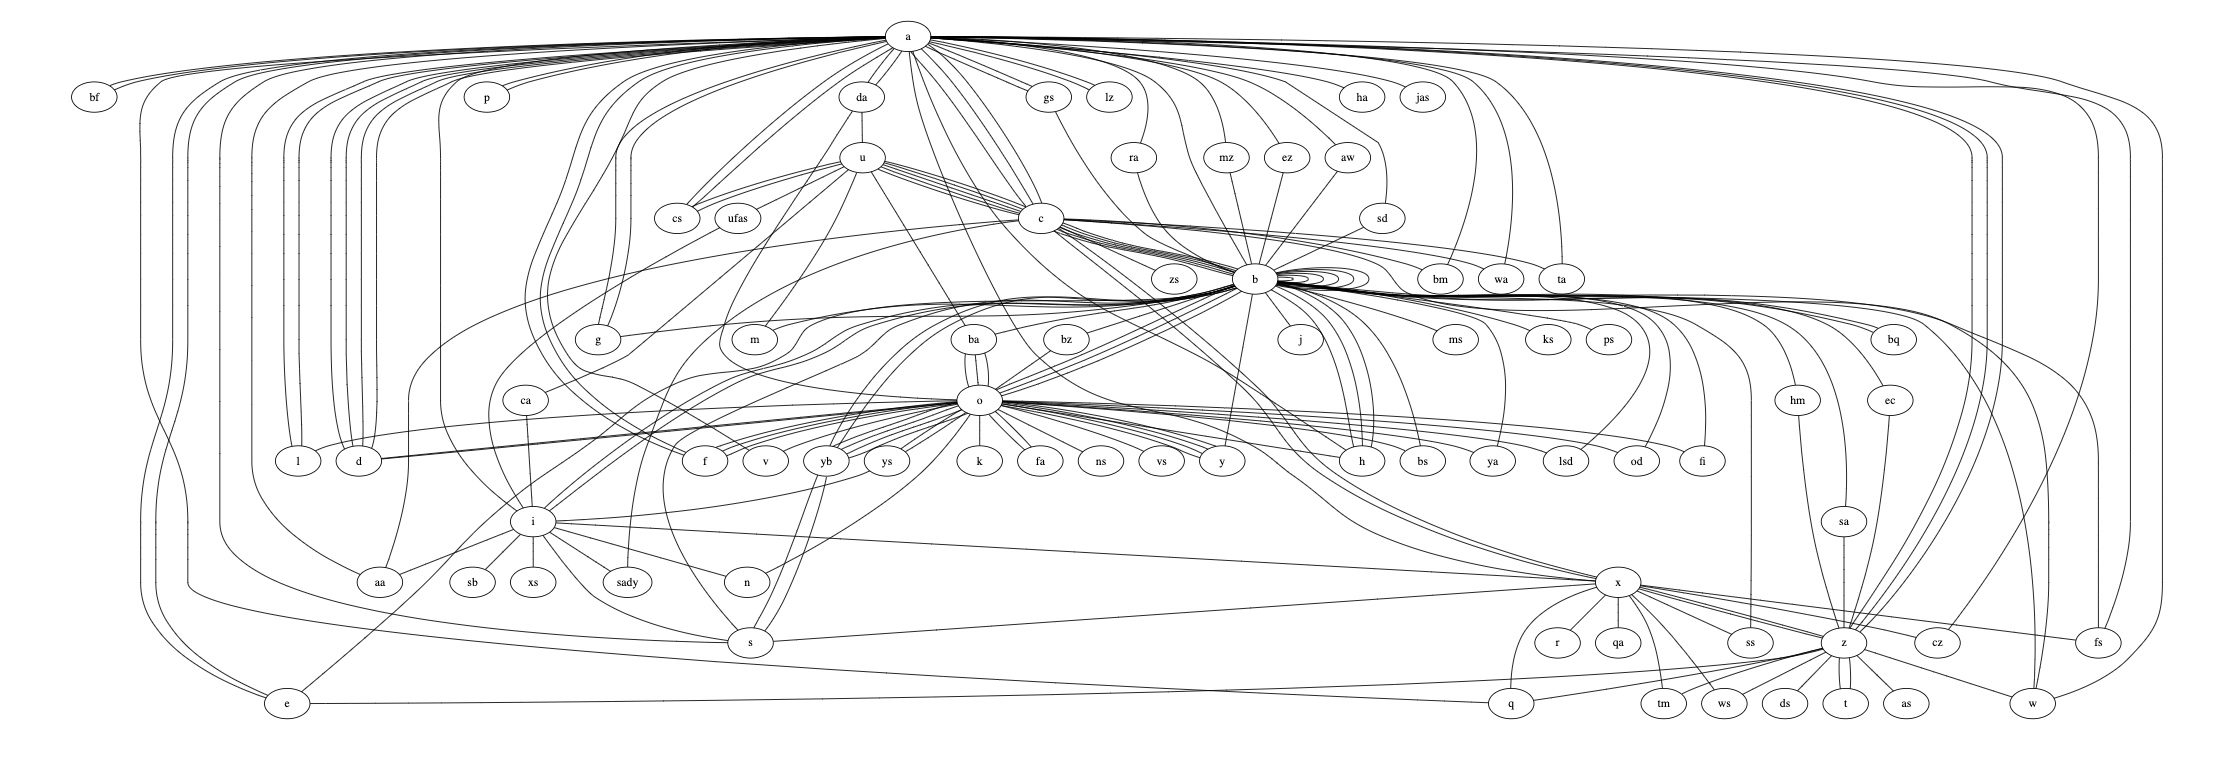
\includegraphics[width=\linewidth]{./../deterministico.png}
  \caption{Automato Finito Determinístico}
  \label{fig:deterministico}
  \end{center}
\end{figure}

%-------------------------------------------------------------------------------

\end{document}
